\documentclass{standalone}
\usepackage{tikz}
\usetikzlibrary{arrows,shapes,automata,positioning,intersections,calc}


\begin{document}
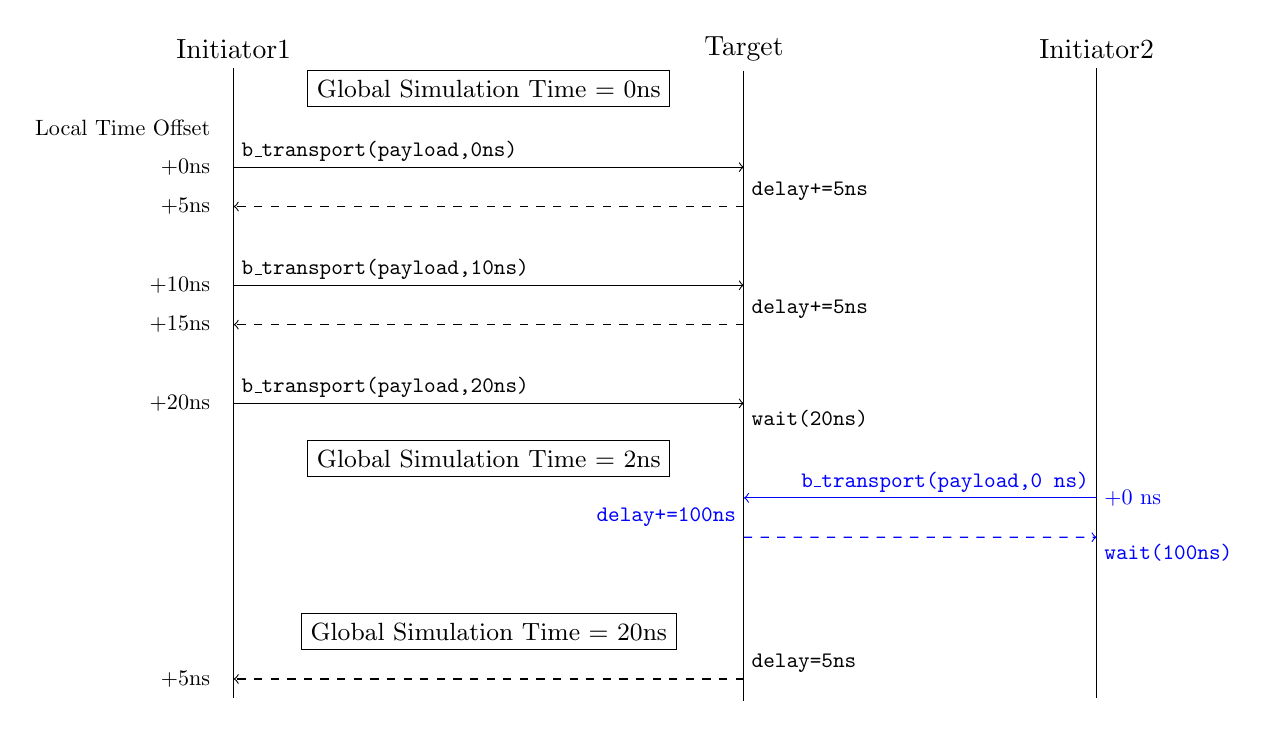
\begin{tikzpicture}

  \node (initiator) {Initiator1};
  \node[right=5cm of initiator] (target) {Target};
  \node[right=3cm of target] (initiator2) {Initiator2};
  \coordinate (a) at ($ (initiator)!.5!(target) $);
  \coordinate (b) at ($ (a) + (0,-5mm) $);
  \coordinate (c) at ($ (a) + (0,-7.4cm) $);
  \coordinate (d) at ($ (a) + (0,-5.2cm) $);
  
  \node[draw] at (b) (time1) {\small Global Simulation Time = 0ns};
  \node[draw] at (d) (time1) {\small Global Simulation Time = 2ns};
  \node[draw] at (c) (time1) {\small Global Simulation Time = 20ns};

  \draw (initiator.south) -- ([yshift=-8cm]initiator.south);
  \draw (target.south)    -- ([yshift=-8cm]target.south);
  \draw (initiator2.south) -- ([yshift=-8cm]initiator2.south);
  
  \coordinate (i1) at ($ (initiator)+(0,-1.5cm) $);
  \coordinate (i2) at ($ (i1)+(0,-5mm) $);  
  \coordinate (i3) at ($ (i2)+(0,-1cm) $);
  \coordinate (i4) at ($ (i3)+(0,-5mm) $);  
  \coordinate (i5) at ($ (i4)+(0,-1cm) $);
  \coordinate (i6) at ($ (i5)+(0,-3.5cm) $);  

  \coordinate (t1) at ($ (target)+(0,-1.5cm) $);
  \coordinate (t2) at ($ (t1)+(0,-5mm) $);  
  \coordinate (t3) at ($ (t2)+(0,-1cm) $);
  \coordinate (t4) at ($ (t3)+(0,-5mm) $);  
  \coordinate (t5) at ($ (t4)+(0,-1cm) $);
  \coordinate (t6) at ($ (t5)+(0,-3.5cm) $);

  \node[anchor=east, scale=0.8] at ([xshift=-2mm,yshift=5mm]i1) {Local Time Offset};

  \foreach \i/\j in {1/0,3/10,5/20}{
    \draw[->] (i\i) node[anchor=east,scale=0.8] at +(-2mm,0) {+\j ns} node[anchor=west,scale=0.8] at +(0,2mm) {\texttt{b\_transport(payload,\j ns)}} -- (t\i);
  }
  
  \node[anchor=west,scale=0.8] at ([yshift=-2mm]t5) {\texttt{wait(20ns)}};

  \foreach \i/\j/\k in {2/5/+=,4/15/+=,6/5/=}{
    \draw[->,dashed] (t\i) node[anchor=west,scale=0.8] at +(0,2mm) {\texttt{delay\k 5ns}} -- (i\i) node[anchor=east,scale=0.8] at +(-2mm,0) {+\j ns};
  }

  \coordinate (j1) at ($ (initiator2)+(0,-5.7cm) $);
  \coordinate (j2) at ($ (initiator2)+(0,-6.2cm) $);
  \coordinate (t7) at ($ (target)+(0,-5.7cm) $);
  \coordinate (t8) at ($ (t7)+(0,-2.5mm) $);
  \coordinate (t9) at ($ (t8)+(0,-2.5mm) $);
  \draw[->,color=blue] (j1) node[anchor=west,scale=0.8]  {+0 ns} node[anchor=east,scale=0.8] at +(0,2mm) {\texttt{b\_transport(payload,0 ns)}} -- (t7);
  \node[color=blue, anchor=east, scale=0.8] at (t8) {\texttt{delay+=100ns}};
  \draw[->,dashed,color=blue] (t9) -- (j2) node[anchor=west,scale=0.8] at +(0,-2mm) {\texttt{wait(100ns)}};

  
\end{tikzpicture}
\end{document}



